\documentclass{article}
\usepackage{graphicx} % Required for inserting images
\usepackage{amsmath}
\usepackage{amssymb}   % Additional symbols, such as \mathbb and various math symbols
\usepackage{amsfonts}  % Additional fonts for mathematical symbols, like \mathbb
\usepackage{mathtools} % Extends amsmath with additional functionality
\usepackage{mathrsfs}  % Provides script fonts (\mathscr)
\usepackage{amsthm}    % Enhanced theorem environments (theorem, lemma, etc.)
\usepackage{bbm}
\usepackage{tikz}
\usetikzlibrary{shapes.geometric, calc}
\usepackage{array}
\usetikzlibrary{intersections, calc}
\usepackage{geometry}


\title{Applied Probability and Statistics I - STAT400}
\author{Tom Mitchell}
\date{Mestiyage - Fall 2024}

\begin{document}

\maketitle

\section*{Syllabus}

\subsection*{Grading}
\begin{itemize}
    \item Homework — 28\% (7\% each)
    \item R Projects — 12\% (4\% each)
    \item Two exams — 30\% (15\% each)
    \item Final exam — 30\%
\end{itemize}

\subsection*{Office Hours}
\begin{itemize}
    \item Tuesday: 1:00 PM - 1:50 PM (in person, MTH 4106)
    \item Wednesday: 11:00 AM - 11:50 AM (online)
\end{itemize}

\subsection*{Exams}
\begin{itemize}
    \item 2 midterms and a final exam
\end{itemize}

\section*{Day 1: Tuesday 8/27/2024}

\section*{Course Overview: STAT400}
We study:
\begin{enumerate}
    \item Probability
    \item Descriptive Statistics
    \item Inferential Statistics
\end{enumerate}

\pagebreak

\subsection*{1. Probability}
\textit{Probability} is the mathematical study of uncertainty.

\subsection*{2. Descriptive Statistics}
\textit{Descriptive Statistics} involves methods for summarizing and describing the important characteristics of a dataset.

\subsection*{3. Inferential Statistics}
\textit{Inferential Statistics} involves methods for using data from a subset (sample) of a larger group (population) to make meaningful conclusions. Note that each time you pick a subset, you lose out on certain information, leading to uncertainty.

\subsection*{Setting: Conducting an Experiment}

In this course, we will often assume we are about to conduct an experiment. The possible outcomes of the experiment are known, but the exact outcome is not.

\textbf{Examples:}
\begin{itemize}
    \item Tossing a coin
    \item Rolling a die
\end{itemize}

To study these types of situations, we introduce a \textit{model for probability}.

\subsection*{Ordered Triples (\(\Omega, \mathcal{F}, P\))}
\begin{itemize}
    \item \(\Omega\) is the \textbf{sample space}: The set of all possible outcomes of the experiment.
    \item \(\mathcal{F}\) is the \textbf{event space}:
    \begin{itemize}
        \item An \textbf{event} is a subset of \(\Omega\).
        \item An event captures the idea that in many situations, we care about collections of outcomes rather than a single outcome.
        \item The event space contains collections of outcomes for which we can assign probabilities.
    \end{itemize}
    \item \(P\) is the \textbf{probability measure}:
    \[
    P: \mathcal{F} \rightarrow \mathbb{R}
    \]
    where \(P\) assigns probabilities to events.

\end{itemize}

\pagebreak

\subsection*{Example 1: Tossing a Fair Coin}
Consider the simple experiment of tossing a \textbf{fair} coin.

\[
\Omega = \{H, T\}
\]

\[
\mathcal{F} = \{\emptyset, \{H\}, \{T\}, \{H, T\}\}
\]

\begin{itemize}
    \item \(P(\emptyset) = 0\) \\
    (``A probability of 0 represents an outcome/collection of outcomes that never takes place.")
    
    \item \(P(\{H, T\}) = 1\) \\
    (``A probability of 1 represents an outcome/collection of outcomes that always takes place.")
    
    \item \(P(\{H\}) = \frac{1}{2}\) \\
    (Requires the coin to be fair.)
    
    \item \(P(\{T\}) = \frac{1}{2}\) \\
    (Requires the coin to be fair.)
\end{itemize}

\subsection*{Example 2: Rolling a Fair Die}
Consider the experiment of rolling a fair die. Note: (\(\mathcal{P}(\Omega)\) is the Powerset of \(\Omega\))

\[
\Omega = \{1, 2, 3, 4, 5, 6\}
\]

\[
\mathcal{F} = \mathcal{P}(\Omega) =
\]
\[
\begin{aligned}
\{\emptyset, \{1\}, \{2\}, \ldots, \{6\}, \{1, 2\}, \ldots, \{1, 6\}, \{2, 3\}, \ldots, \\
\{1, 2, 3\}, \{2, 3, 4\}, \ldots, \{1, 2, 3, 4\}, \{1, 2, 3, 4, 5\}, \ldots, \Omega = \{1, 2, 3, 4, 5, 6\}\}
\end{aligned}
\]

\begin{itemize}
    \item \(P(\{i\}) = \frac{1}{6}\) for \(i = 1, 2, 3, 4, 5, 6\)
    \item \(P(\emptyset) = 0\)
    \item \(P(\Omega) = 1\)
    \item \(P(\{1, 2\}) = ?\) \\
    (Listing out probabilities for each event is \textbf{not} feasible.)
\end{itemize}

We would want a way to calculate the probability of a particular event by using the ``base" probabilities.

\textit{We will look at these rules for computing probabilities of complicated events in terms of basic ones in a bit.}

\subsection*{Example 3: Tossing a Fair Coin Until We See Heads for the First Time}
Consider the experiment of tossing a fair coin repeatedly until we observe heads for the first time, then we stop.

\[
\Omega = \{(H), (T, H), (T, T, H), (T, T, T, H), \ldots\}
\]

\[
\mathcal{F} = \mathcal{P}(\Omega)
\]

Let \(A_i\) be the event of seeing heads on the \(i\)th toss.

\[
P(A_i) = \frac{1}{2^i}
\]

\textbf{Question:} What is the probability of seeing heads on an even-numbered toss?

\[
Q = P(\text{seeing heads on an even-numbered toss}) = ?
\]

\subsection*{Example 4: Picking a Number from the Interval [0, 1]}
Consider picking a number from the interval \([0, 1]\) such that the probabilities of selecting numbers from two subintervals \(I_1\) and \(I_2\) of \([0, 1]\) are the same whenever \(I_1\) and \(I_2\) have the same length.

\[
\Omega = [0, 1]
\]

\[
\mathcal{F} = \mathcal{P}(\Omega)
\]

\[
P(\text{selecting a number from a subinterval } I \text{ of } [0, 1]) = \text{length}(I)
\]

\[
P([0, \frac{1}{4}]) = \frac{1}{4} - 0 = \frac{1}{4}
\]

\[
P([0, \frac{1}{2}]) = \frac{1}{2} - 0 = \frac{1}{2}
\]

\[
P\left(\left\{\frac{1}{2}\right\}\right) = P\left(\left[\frac{1}{2}, \frac{1}{2}\right]\right) = \frac{1}{2} - \frac{1}{2} = 0
\]

``The probability of 0 indicates an event that does not take place or an event that is so unlikely that the only reasonable value to assign to it is 0, i.e., an event that almost surely does not take place."

On Thursday will learn how to compute problems similar to \(P(\mathbb{Q} \cap [0, 1])\) = ?


\pagebreak

\section*{Day 2: Thursday 8/29/2024}

\subsection*{Probability}

\begin{itemize}
    \item Mathematical study of uncertainty.
\end{itemize}

\subsection*{Probability Space}

\[
(\Omega, F, P)
\]

\begin{itemize}
    \item \(\Omega\) - All possible outcomes of the experiment of interest.
    \item \(F\) - Contains events, i.e., collections of outcomes we would like to assign probabilities to.
    \item \(P\) - Probability measure.
\end{itemize}

\[
P: F \rightarrow \mathbb{R}
\]

On Tuesday, we discussed examples and introduced some formulas to compute probabilities of ``basic" events.

\subsection*{Goal for Today}

Explore how to compute probabilities of ``complicated" events in terms of basic events.

\subsection*{Two Questions}

\begin{enumerate}
    \item How do we express a complicated event in terms of basic ones?
    \item What rules can be used to compute probabilities once Question 1 has been answered?
\end{enumerate}

\begin{itemize}
    \item Question 1 is best answered by using tools from set theory.
\end{itemize}

\[
\rightarrow \text{We treat } \Omega \text{ as the list of all possible outcomes.}
\]
\[
\rightarrow \text{Events are sublists of } \Omega.
\]

Since we are only interested in outcomes (or combinations thereof) of the experiment, we treat \(\Omega\) as the universal set (i.e., we pretend that nothing outside of \(\Omega\) exists).

\subsection*{Pictorial Representation}

\begin{center}
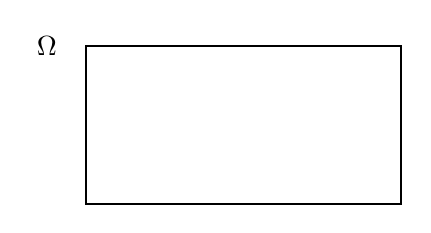
\begin{tikzpicture}
    \draw[thick] (0,0) rectangle (4,2);
    \node at (-0.5,2) {\(\Omega\)};
\end{tikzpicture}
\end{center}

\pagebreak

We can manipulate collections of events to obtain new events in various ways:

\begin{itemize}
    \item Intersections
    \item Unions
    \item Relative complements
\end{itemize}

Given events \(A\) and \(B\), the intersection is the event that contains all outcomes common to both \(A\) and \(B\). We denote this by \(A \cap B\).

\subsection*{Intersection of Two Events}

\begin{center}
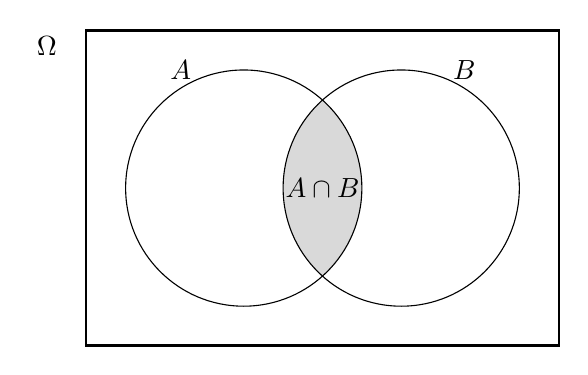
\begin{tikzpicture}
    % Draw the rectangle representing the universal set Omega
    \draw[thick] (-2,-2) rectangle (4,2);
    \node at (-2.5,1.8) {\(\Omega\)};
    
    % Draw the circles representing sets A and B
    \begin{scope}
        \clip (0,0) circle(1.5);
        \fill[gray!30] (2,0) circle(1.5);
    \end{scope}
    \draw (0,0) circle(1.5);
    \draw (2,0) circle(1.5);
    
    % Label the sets
    \node at (-0.8,1.5) {\(A\)};
    \node at (2.8,1.5) {\(B\)};
    
    % Label the intersection area
    \node at (1,0) {\(A \cap B\)};
    
\end{tikzpicture}
\end{center}

\subsection*{Example}

\[
\Omega = \{1, 2, 3, 4, 5, 6\}
\]

Let \(A = \{1, 3, 5\}\) and \(B = \{4, 5\}\). Then, the intersection of \(A\) and \(B\) is:

\[
A \cap B = \{5\}
\]

\subsection*{Extending the Intersection to Families of Events}

The idea of the intersection of events can be extended to families of events.

\[
\bigcap_{i=1}^{3} A_i = (A_1 \cap A_2) \cap A_3
\]

For an infinite family of events:

\[
\bigcap_{i=1}^{\infty} A_i = A_1 \cap A_2 \cap A_3 \cap A_4 \cap A_5 \cap \ldots
\]


\subsection*{Disjoint Events}

Two events are said to be disjoint if \(A \cap B = \emptyset\).

\begin{itemize}
    \item Events \(A_1, \ldots, A_n\) are said to be disjoint if \(\textstyle \bigcap_{i=1}^{n} A_i = \emptyset \).

    \item Events \(A_1, \ldots, A_n, \ldots\) are said to be disjoint if \(\textstyle \bigcap_{i=1}^{\infty} A_i = \emptyset \).
 
    \item Events \(A_1, A_2, \ldots\) are said to be pairwise disjoint if \(A_i \cap A_j = \emptyset\) for all \(i \neq j\).
\end{itemize}

\subsection*{Example}

Consider the sample space \(\Omega = \{1, 2, 3, 4, 5, 6\}\) with the following events:

\[
A = \{1, 3, 5\}, \quad B = \{4, 5\}, \quad C = \{6\}
\]

Here, \(A\), \(B\), and \(C\) are disjoint events, meaning:

\[
A \cap B \cap C = \emptyset
\]

However, they are not pairwise disjoint, because:

\[
A \cap B = \{5\} \neq \emptyset
\]

\subsection*{Pairwise Disjoint Sets}

\begin{center}
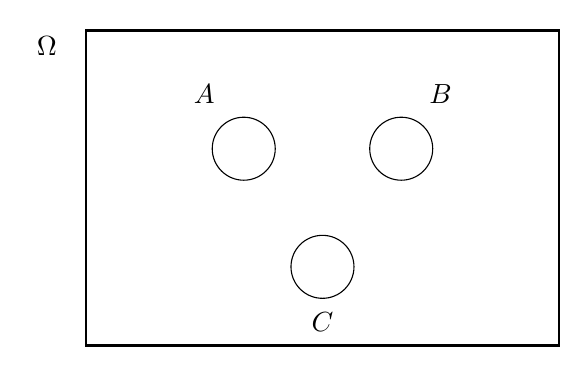
\begin{tikzpicture}

    % Draw the rectangle representing the universal set Omega
    \draw[thick] (-2,-2) rectangle (4,2);
    \node at (-2.5,1.8) {\(\Omega\)};
    
    % Draw non-intersecting circles representing pairwise disjoint sets
    \draw (0,0.5) circle(0.4);
    \draw (2,0.5) circle(0.4);
    \draw (1,-1) circle(0.4);
    
    % Label the sets
    \node at (-0.5,1.2) {\(A\)};
    \node at (2.5,1.2) {\(B\)};
    \node at (1,-1.7) {\(C\)};
    
\end{tikzpicture}
\end{center}


The word ``and" usually translates to intersection when discussing sets or events. Conversely, the word ``or" translates to a union.

\subsection*{Unions}

The union of two events \(A\) and \(B\), denoted by \(A \cup B\), is the event that contains all outcomes that are in \(A\), \(B\), or both.

\subsection*{Venn Diagram: Union of Two Sets}

\begin{center}
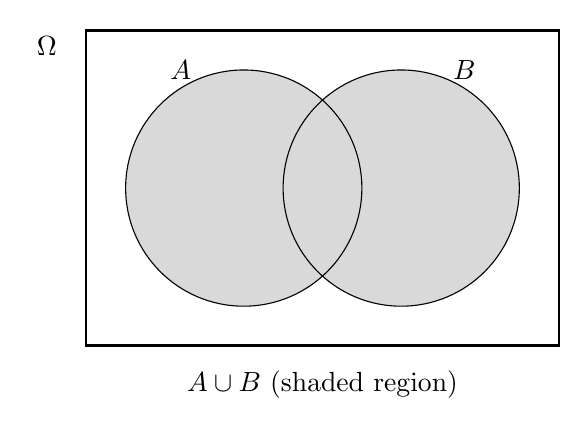
\begin{tikzpicture}

    % Draw the rectangle representing the universal set Omega
    \draw[thick] (-2,-2) rectangle (4,2);
    \node at (-2.5,1.8) {\(\Omega\)};
    
    % Draw the circles representing sets A and B
    \begin{scope}
        \clip (0,0) circle(1.5);
        \fill[gray!30] (2,0) circle(1.5);
    \end{scope}
    \fill[gray!30] (0,0) circle(1.5);
    \fill[gray!30] (2,0) circle(1.5);
    \draw (0,0) circle(1.5);
    \draw (2,0) circle(1.5);
    
    % Label the sets
    \node at (-0.8,1.5) {\(A\)};
    \node at (2.8,1.5) {\(B\)};
    \node at (1,-2.5) {\(A \cup B\) (shaded region)};
    
\end{tikzpicture}
\end{center}

\subsection*{Example}

Consider the sample space \(\Omega = \{1, 2, 3, 4, 5, 6\}\) with the following events:

\[
A = \{1, 3, 5\}, \quad B = \{2, 3, 5\}
\]

The union of \(A\) and \(B\) is:

\[
A \cup B = \{1, 2, 3, 5\}
\]


\subsection*{Infinite and Finite Unions}

Infinite versions of unions and finite versions of unions with more than two sets can be similarly defined.

\[
\bigcup_{i=1}^{3} A_i = A_1 \cup A_2 \cup A_3
\]

Similarly, the union of more than two finite sets can be defined as:

\[
\bigcup_{i=1}^{n} A_i = A_1 \cup A_2 \cup \ldots \cup A_n
\]

Unions can also be extended to infinite collections of sets. For example, the union of an infinite sequence of sets \(A_1, A_2, \ldots\) is denoted as:

\[
\bigcup_{i=1}^{\infty} A_i = A_1 \cup A_2 \cup \ldots
\]



\subsection*{Relative Complements}

Given events \(A\) and \(B\), the relative complement \(A - B\) is the event that contains only the outcomes that are \textbf{unique} to \(A\).

\subsection*{Venn Diagram: Unique to A (\(A - B\))}

\begin{center}
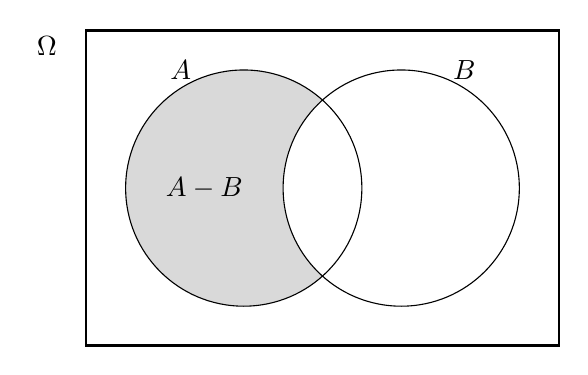
\begin{tikzpicture}

    % Draw the rectangle representing the universal set Omega
    \draw[thick] (-2,-2) rectangle (4,2);
    \node at (-2.5,1.8) {\(\Omega\)};
    
    % Draw the circles representing sets A and B
    \fill[gray!30] (0,0) circle(1.5);
    \begin{scope}
        \clip (2,0) circle(1.5);
        \fill[white] (0,0) circle(1.5);
    \end{scope}
    \draw (0,0) circle(1.5);
    \draw (2,0) circle(1.5);
    
    % Label the sets
    \node at (-0.8,1.5) {\(A\)};
    \node at (2.8,1.5) {\(B\)};
    \node at (-0.5,0) {\(A - B\)};
    
\end{tikzpicture}
\end{center}

\subsection*{Example}

Consider the sample space \(\Omega = \{1, 2, 3, 4, 5, 6\}\) with the following events:

\[
A = \{1, 2, 3\}, \quad B = \{2, 4, 5\}
\]

The relative complements are:

\[
A - B = \{1, 3\}, \quad B - A = \{4, 5\}
\]


\subsection*{Complement of A}

We use \(A^c\) to denote the complement of \(A\) within the universal set \(\Omega\), which is the set of outcomes that are not in \(A\):

\[
A^c = \Omega - A = \{4, 5, 6\}
\]

The word \textbf{not} is associated with complements and the phrases ``and not", ``but not" are associated with relative compliments

\subsection*{Aside (for the HW): Verifying Set Identities with Venn Diagrams}

We can use Venn diagrams to verify set identities. For example, let's verify the identity:

\[
(A \cap B)^c = A^c \cup B^c
\]

Venn diagrams representing set operations of (left hand side) LHS and (right hand side) RHS respectively are shown below:

\begin{figure}[htbp]
\centering
\begin{tikzpicture}
    \node at (0, 3) {\textbf{LHS}};
    \node at (7, 3) {\textbf{RHS}};
    % Left Column - Top (A \cap B)
    \node at (0, 0) {
        \begin{tikzpicture}
            \node at (1,2.5) {\(A \cap B\)};
            % Draw the rectangle representing the universal set Omega
            \draw[thick] (-2,-2) rectangle (4,2);
            
            % Draw A and B with intersection filled
            \begin{scope}
                \clip (0,0) circle(1.5);
            \end{scope}
            \begin{scope}
                \clip (2,0) circle(1.5);
                \fill[gray!30] (0,0) circle(1.5);
            \end{scope}
            \draw (0,0) circle(1.5);
            \draw (2,0) circle(1.5);
            
            % Label the sets
            \node at (-0.8,1.5) {\(A\)};
            \node at (2.8,1.5) {\(B\)};
        \end{tikzpicture}
    };

    % Left Column - Bottom (Complement of A \cap B)
    \node at (0, -6) {
        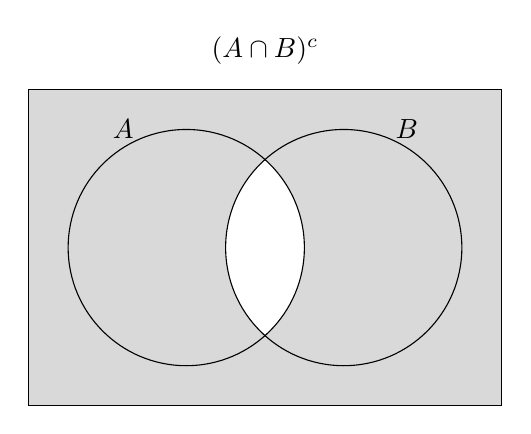
\begin{tikzpicture}
            \node at (1,2.5) {\((A \cap B)^c\)};
            % Draw the rectangle representing the universal set Omega
            \draw[thick] (-2,-2) rectangle (4,2);
            
            % Draw (A \cap B)^c
            \fill[gray!30] (-2,-2) rectangle (4,2);
            \begin{scope}
                \clip (0,0) circle(1.5);
            \end{scope}
            \begin{scope}
                \clip (2,0) circle(1.5);
                \fill[white!30] (0,0) circle(1.5);
            \end{scope}
            \draw (0,0) circle(1.5);
            \draw (2,0) circle(1.5);
            
            % Label the sets
            \node at (-0.8,1.5) {\(A\)};
            \node at (2.8,1.5) {\(B\)};
        \end{tikzpicture}
    };

    % Right Column - Top (A^c)
    \node at (7, 0) {
        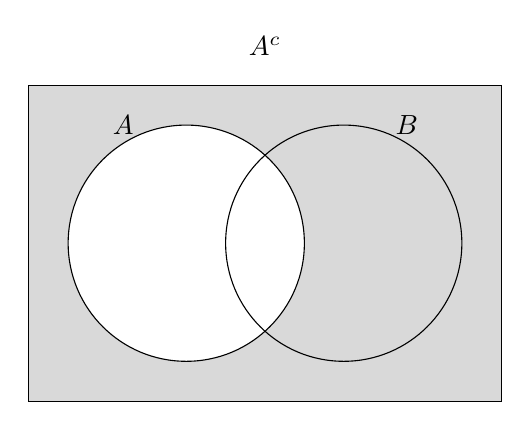
\begin{tikzpicture}
            \node at (1,2.5) {\(A^c\)};
            % Draw the rectangle representing the universal set Omega
            \draw[thick] (-2,-2) rectangle (4,2);
            
            % Draw complement of A
            \fill[gray!30] (-2,-2) rectangle (4,2);
            \fill[white] (0,0) circle(1.5);
            \draw (0,0) circle(1.5);
            \draw (2,0) circle(1.5);
            
            % Label the sets
            \node at (-0.8,1.5) {\(A\)};
            \node at (2.8,1.5) {\(B\)};
        \end{tikzpicture}
    };

    % Right Column - Middle (B^c)
    \node at (7, -6) {
        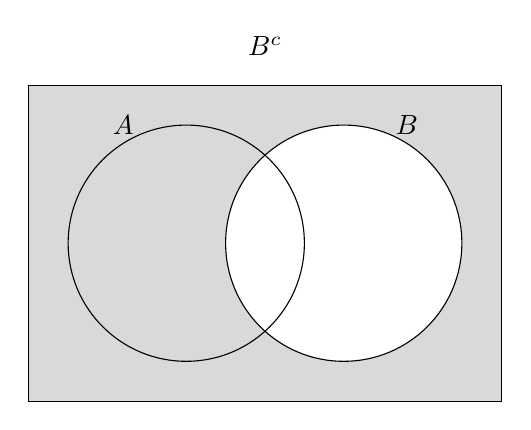
\begin{tikzpicture}
            \node at (1,2.5) {\(B^c\)};
            % Draw the rectangle representing the universal set Omega
            \draw[thick] (-2,-2) rectangle (4,2);
            
            % Draw complement of B
            \fill[gray!30] (-2,-2) rectangle (4,2);
            \fill[white] (2,0) circle(1.5);
            \draw (0,0) circle(1.5);
            \draw (2,0) circle(1.5);
            
            % Label the sets
            \node at (-0.8,1.5) {\(A\)};
            \node at (2.8,1.5) {\(B\)};
        \end{tikzpicture}
    };

    % Right Column - Bottom (A^c \cup B^c)
    \node at (7, -12) {
        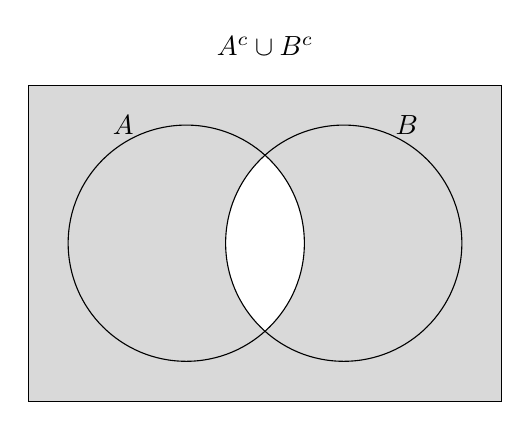
\begin{tikzpicture}
            \node at (1,2.5) {\(A^c \cup B^c\)};
            % Draw the rectangle representing the universal set Omega
            \draw[thick] (-2,-2) rectangle (4,2);
            
            % Draw A^c union B^c
            \fill[gray!30] (-2,-2) rectangle (4,2);
            \begin{scope}
                \clip (0,0) circle(1.5);
            \end{scope}
            \begin{scope}
                \clip (2,0) circle(1.5);
                \fill[white!30] (0,0) circle(1.5);
            \end{scope}
            \draw (0,0) circle(1.5);
            \draw (2,0) circle(1.5);
            
            % Label the sets
            \node at (-0.8,1.5) {\(A\)};
            \node at (2.8,1.5) {\(B\)};
        \end{tikzpicture}
    };

\end{tikzpicture}
\label{fig:venn-diagrams}
\end{figure}


\pagebreak

\subsubsection*{Conclusion}

Both sides of the identity are visually represented by the same shaded region, thus confirming that:

\[
(A \cap B)^c = A^c \cup B^c
\]


The shaded regions for \((A \cap B)^c\) and \(A^c \cup B^c\) match. Therefore, \((A \cap B)^c = A^c \cup B^c\). 

\[\]

\textbf{Note}: (we are not worrying about edges cases, for example, where A and B are disjoint but the identity still holds true)

\[\]
Now that the terminology is in place, we start to answer Q2.

\section*{Axioms}

\begin{enumerate}
    \item \(P(\Omega) = 1\), \(P(\emptyset) = 0\)
    \item \(P(A) \geq 0 \quad \text{for all } A \in \mathcal{F}\)
    \item If \(A_1, A_2, \ldots, A_n, \ldots \in \mathcal{F}\) are pairwise disjoint, then 
    \[
    P\left(\bigcup_{i=1}^{\infty} A_i\right) = \sum_{i=1}^{\infty} P(A_i)
    \]
\end{enumerate}


\textbf{Example:}
Consider the problem of tossing a fair coin until we observe heads. We want to find P(heads on an even numbered toss)

Let \( A \) be the event that heads appears for the first time on an even-numbered toss.

Thus, \( A \) can be expressed as:
\[
A = \{ (T, H), (T, T, T, H), (T, T, T, T, T, H), \dots \}
\]

Recall, $A_i$ is heads on the ith toss.


\[
P(A_i) = \frac{1}{2^i}
\]


Notice that we can describe \( A \) as the union of disjoint events where heads occurs for the first time on the \( 2i \)-th toss:

\[
A = A_2 \cup A_4 \cup A_6 \cup \dots = \bigcup_{i=1}^{\infty} A_{2i}
\]

where \( A_{2i} \) is the event that heads first appears on the \( 2i \)-th toss. The probability of \( A_{2i} \) can be computed as:
\[
P(A_{2i}) = \left(\frac{1}{2}\right)^{2i}
\]

Since the events \( A_{2i} \) are pairwise disjoint, we can use axiom 3 to see the probability of \( A \) is given by:
\[
P(A) = P\left(\bigcup_{i=1}^{\infty} A_{2i}\right)
= \sum_{i=1}^{\infty} P(A_{2i}) 
= \sum_{i=1}^{\infty} \left(\frac{1}{2}\right)^{2i} = \sum_{i=1}^{\infty} \left(\frac{1}{4}\right)^{i}
\]
This series is an infinite geometric series with the first term \( a = \frac{1}{4} \) and common ratio \( r = \frac{1}{4} \): 

Recall, that a the sum of a converging infinite geometric series where \(|r| < 1\) is:
\[
S = a+ar+ar^2+... = \sum_{i=0}^{\infty} \left(ar^n\right) = \frac{a}{1 - r}
\]

Therefore:
\[
\sum_{i=1}^{\infty} \left(\frac{1}{4}\right)^i = \frac{\frac{1}{4}}{1 - \frac{1}{4}} = \frac{\frac{1}{4}}{\frac{3}{4}} = \frac{1}{3}
\]

Thus, the probability that the first occurrence of heads is on an even-numbered toss is \( \boxed{\frac{1}{3}} \).


Derived rule: If \( A_1, \dots, A_N \in \mathcal{F} \) are pairwise disjoint, then 
\[
P\left(\bigcup_{i=1}^{\infty} A_i\right) = \sum_{i=1}^{\infty} P(A_i)
\]

\textbf{Example}: Consider a fair die roll. What is the probability of rolling a 1, 3, or 5?

\[
P(\{i\}) = \frac{1}{6} \quad \text{for } i = 1, \dots, 6
\]

\[
P(\{1, 3, 5\}) = P(\{1\}) + P(\{3\}) + P(\{5\}) = \frac{1}{6} + \frac{1}{6} + \frac{1}{6} = \frac{1}{2}
\]































\end{document}
